% *********************************************************************
% © 2016–2025 Jeremy Sylvestre
%
% Permission is granted to copy, distribute and/or modify this document
% under the terms of the GNU Free Documentation License, Version 1.3 or
% any later version published by the Free Software Foundation; with no
% Invariant Sections, no Front-Cover Texts, and no Back-Cover Texts. A
% copy of the license is included in the appendix entitled “GNU Free
% Documentation License” that appears in the output document of this
% PreTeXt source code. All trademarks™ are the registered® marks of
% their respective owners.
%
% *********************************************************************
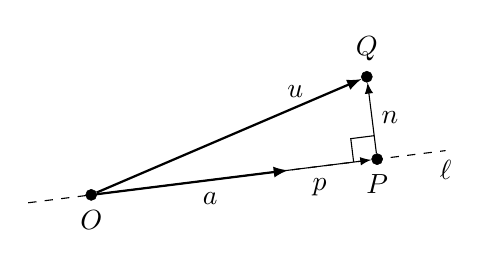
\begin{tikzpicture}[
	point/.style={circle,draw,very thin,fill,inner sep=0pt,minimum size=4pt},
	vector/.style={-latex},
]
	% line slope 1/8, perp slope = -8
	\coordinate (l1) at (-0.8,-0.1);
	\coordinate (l2) at (4.5,0.5625);
	\draw[dashed] (l1) to node[below,at end] {$\ell$} (l2);

	\node[point] at (0,0) (o) [label=below:{$O$}] {};
	\node[point] at (3.5,1.5) (u) [label=above:{$Q$}] {};
	\node[point] at (3.631,0.454) (p) [label=below:{$P$}] {};
	\draw[vector,thick] (o) to node[above,near end] {$\uvec{u}$} (u);
	\draw[vector,thick] (o) to node[below right] {$\uvec{a}$} (2.5,0.3125); % parallel to (2,0.25)
	\draw[vector] (o) to node[below right,near end] {$\uvec{p}$} (p);
	\draw[vector] (p) to node[right] {$\uvec{n}$} (u);

	% perp square
	\draw (3.594,0.752) to (3.296,0.714) to (3.333,0.417);

\end{tikzpicture}
